\chapter{Estado da Arte}
\label{ch::estado-arte}

\section{Introdução}
\label{sec::estado-arte:intro}

O que é a holografia? O que é um holograma? Como se obtêm, codificam e representam? Que formas já foram estudadas de os comprimir? Como se pode avaliar a qualidade da imagem comprimida?

Estas e outras questões impõem-se perante a investigação que se almeja. A sua resposta, dada no presente Capítulo, orientará a definição de uma estratégia de investigação e permitirá avançar a área da holografia com um renovado conhecimento acerca da compressão de hologramas com a norma JPEG2000.

% ----------------------------------------------------------------------------------------
\section{Perspetiva Histórica e Conceitos Base da Holografia}
\label{sec::estado-arte:hist-base}

% O que é um holograma
Entende-se por \textbf{holograma} uma gravação física de um padrão de interferência que recorre ao efeito de difração da luz para reproduzir um campo de luz tridimensional. Tal resulta numa imagem a qual retém as propriedades da cena original, entre elas a profundidade e a paralaxe\cite{holocenter}.

Por seu turno, a \textbf{holografia} é a ciência envolvida no estudo da obtenção de hologramas.

Há a referir brevemente os seguintes conceitos para clarificação:
\begin{itemize}
  \item \textbf{Difração}: Conjunto de fenómenos que ocorrem quando uma onda encontra um obstáculo, em particular a sua aparente flexão e alargamento ao atravessar orifícios\cite{Grimaldi2010,Cajori1929};
  \item \textbf{Interferência}: Semelhante à difração, mas referente à sobreposição de duas ou mais ondas;
  \item \textbf{Paralaxe}: Diferença na posição aparente de um objeto quando observado em locais diferentes\cite{stevenson2007shorter,waite2013pocket}.
\end{itemize}


\begin{figure}[!htbp]
  \centering
  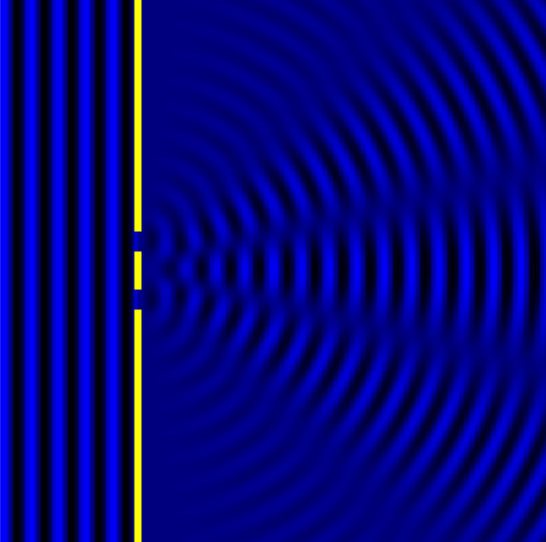
\includegraphics[width=0.5\textwidth]{Doubleslit}
  \caption[Ilustração do efeito de difração.]{Ilustração do efeito de difração de uma onda a atravessar dois orifícios vizinhos\cite{img:doubleslit}.}
  \label{fig:diffraction}
\end{figure}

\begin{figure}[!htbp]
  \centering
  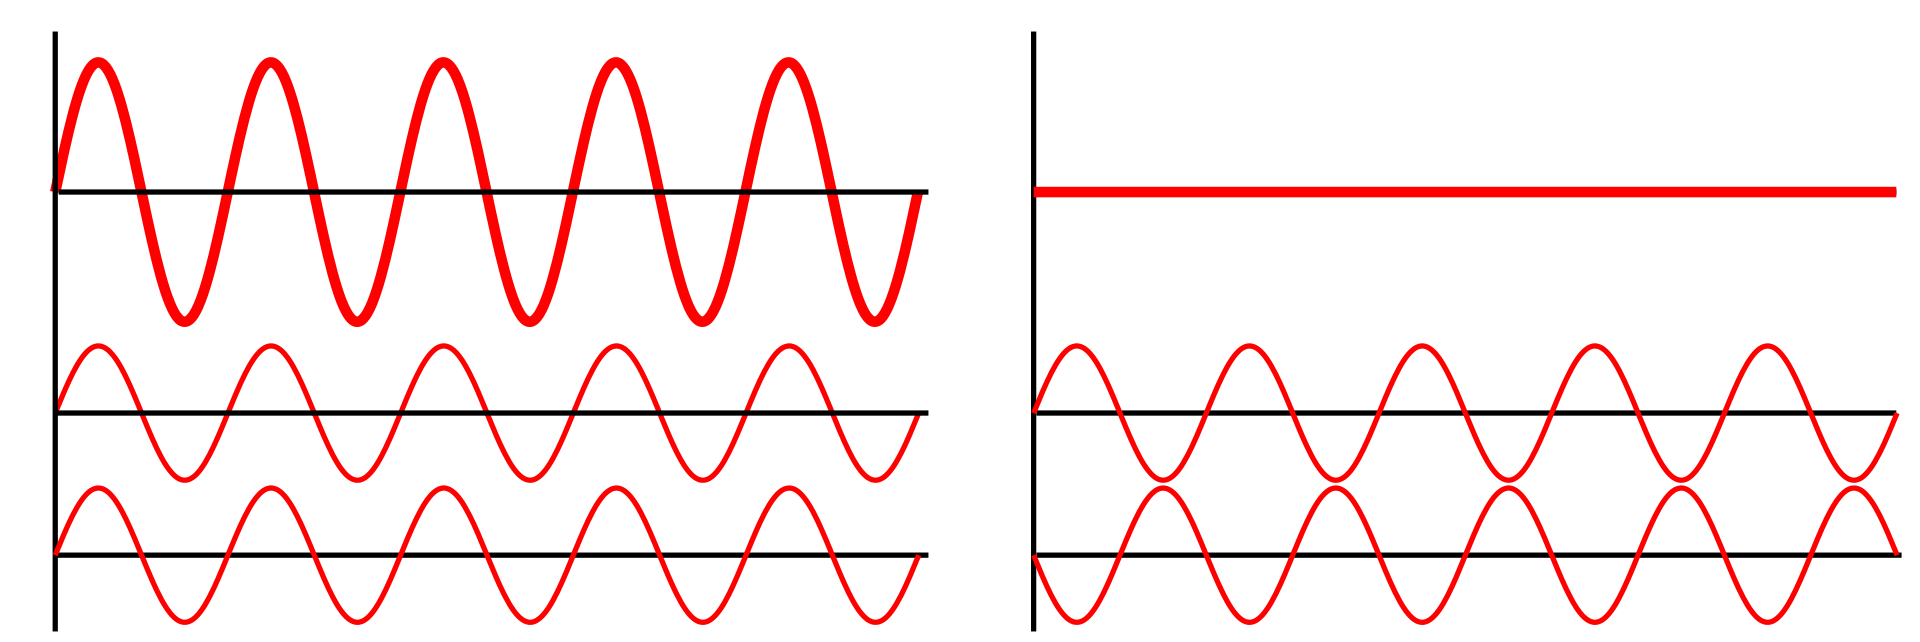
\includegraphics[width=\textwidth]{Interference}
  \caption[Ilustração do efeito de interferência.]{Ilustração do efeito de interferência de duas ondas\cite{img:interference}. Do lado esquerdo encontra-se representada uma interferência construtiva: as duas ondas sincronizadas (\textit{i.e.} exatamente em fase) produzem uma nova onda de amplitude aumentada. Do lado direito apresenta-se um caso de interferência destrutiva: existe uma anulação das ondas por estarem exatamente fora de fase.}
  \label{fig:interference}
\end{figure}

\begin{figure}[!htbp]
  \centering
  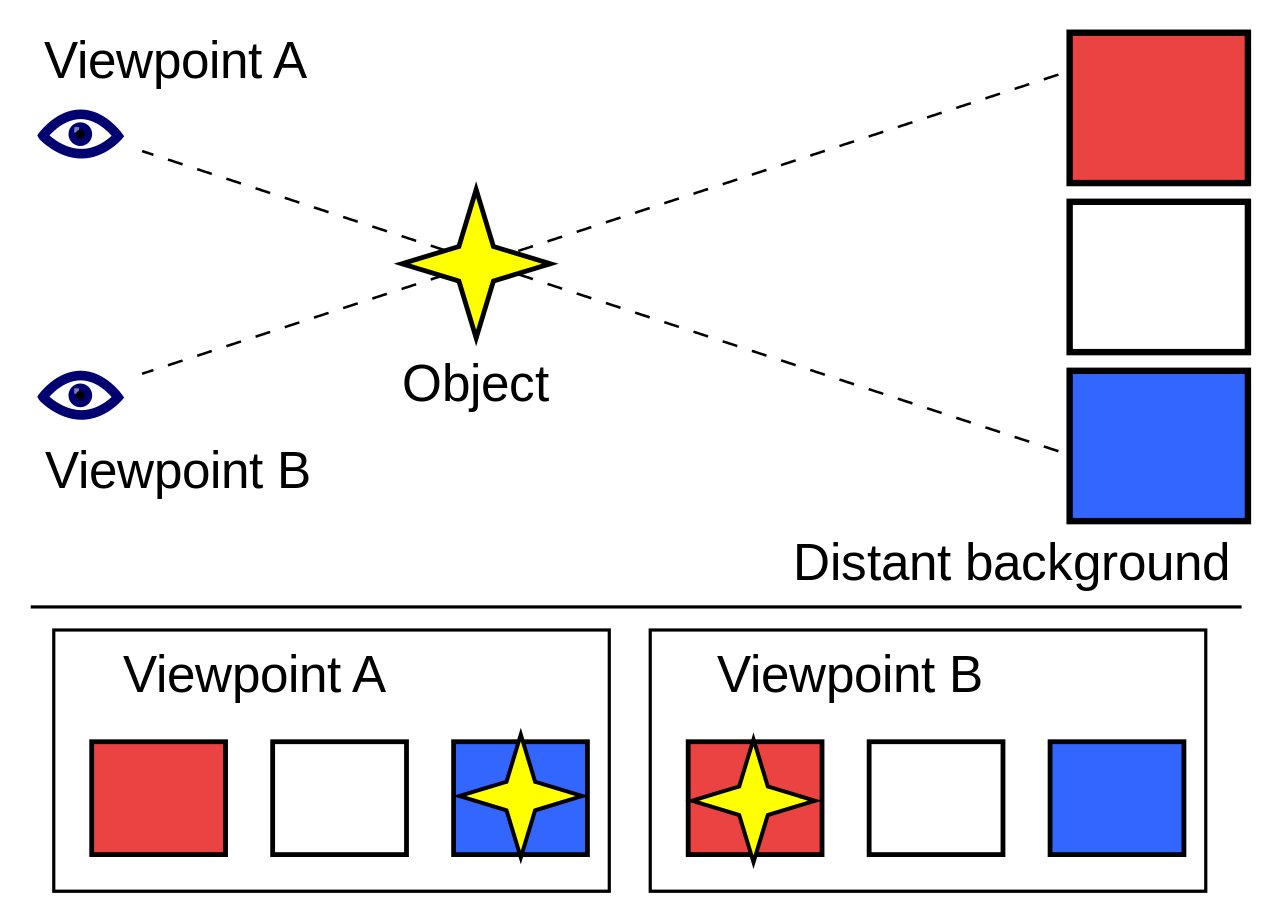
\includegraphics[width=0.6\textwidth]{parallax}
  \caption[Ilustração do efeito de paralaxe.]{Ilustração do efeito de paralaxe de um objeto face a um padrão de fundo\cite{img:parallax}. Devido à mudança de perspetiva do utilizador em dois pontos de vista distintos, no ponto A o observador perceciona a estrela como estando sobre o fundo azul, enquanto no ponto B esta aparenta estar sobre o fundo vermelho.}
  \label{fig:parallax}
\end{figure}


Enquanto a fotografia tradicional apenas captura a intensidade da luz refletida pelos objetos, a holografia permite capturar tanto a amplitude como a fase da onda de luz dispersa por um objeto\cite{holocenter,Image2018,spencer1973the}.

Em contraste face à fotografia clássica, a qual teve as suas origens desde a descoberta da \textit{camara obscura} por parte da China Antiga\cite{Krebs2004}, a holografia como ciência conheceu o seu início com o cientista húngaro-britânico Dennis Gabor na década de 1940 enquanto este estudava avanços na tecnologia da microscopia eletrónica\cite{GABOR1948, GABOR1949}. A descoberta da holografia e, por sua vez, dos hologramas foi inesperada.

A técnica foi adaptada e é ainda hoje utilizada na microscopia eletrónica no que se chama de \textbf{holografia eletrónica}. Contudo, a \textbf{holografia ótica} só pôde avançar após a invenção do \textit{laser} na década de 1960\cite{Leith1962,Leith1964}.

O ponto-chave no desenvolvimento de imagens holográficas, proposto por Dennis Gabor em 1948 numa tentativa de melhorar a microscopia eletrónica, é o uso de uma fonte de luz de referência para codificar uma onda sobreposta com outra a fim de registar os padrões de interferência\cite{GABOR1948}. Contudo, as experiências de Gabor eram limitadas pelo uso de ondas óticas paralelas ao eixo ótico\cite{Image2018}.

Desta forma, em 1962, Emmet Leith e Juris Upatnieks desenvolveram a técnica que viria a lançar em definitivo a holografia ótica: a \textbf{holografia ótica \textit{off-axis}}\cite{Leith1962}, ou seja, o eixo ótico não é paralelo ao feixe de ondas óticas. Esta técnica, desenvolvida no âmbito do estudo de radares, teve a sua prova prática após a invenção do \textit{laser} e, em 1964, os dois cientistas produziram uma série de hologramas que culminariam na atribuição do Prémio Nóbel da Física a Dennis Gabor em 1971\cite{Leith1962,nobel1971}.

Diferentes tipos de hologramas óticos foram desenvolvidos nas décadas subsequentes, assim como outras áreas beneficiaram com os estudos enveredados na área da holografia\cite{Image2018}. Em particular, o desenvolvimento de hologramas visualizados pela transmissão de luz branca, por Stephen Benton\cite{benton1977}, permitiu avanços na medicina, em particular na área da imagiologia, onde a holografia foi incorporada em exames como a \ac{TAC} e a \ac{RMN}\cite{Saxon2003}. Curiosamente, esta técnica é comummente vista em cartões de crédito/débito e documentos de identificação nacional oficiais\cite{Saxon2003,Toal2012}.




\section{O Holograma}
\label{sec::estado-arte:holograma}

Existem atualmente duas formas de obter e reconstruír hologramas\cite{Image2018}:
\begin{enumerate}
  \item Configuração \textbf{analógica} (método original);
  \item Configurações \textbf{digitais}.
\end{enumerate}

De notar que existem diferentes métodos tanto para a obtenção como para a reconstrução numérica na holografia digital (Figura \ref{fig:holografia}).

A \textbf{holografia digital} em particular é um processo de três passos\cite{Image2018}:
\begin{enumerate}
  \item Geração do campo de ondas do objeto;
  \item Aquisição (ou registo) do padrão de interferência;
  \item Reconstrução do campo do objeto para visualização tridimensional ou em multivista bidimensional renderizada.
\end{enumerate}

As configurações digitais serão as abordadas na presente Secção, sendo a analógica ignorada, uma vez que ambas apresentam princípios teóricos semelhantes e o âmbito do projeto é a holografia digital. Em particular, serão abordadas apenas as técnicas utilizadas na obtenção e reconstrução dos hologramas testados no projeto.


\subsection{Obtenção}
\label{ssec::estado-arte:holograma:obter}

A obtenção de um holograma envolve a codificação da amplitude e da fase da onda de luz dispersa por um objeto. Esta varia conforme o meio onde o holograma será gravado. Uma vez que os métodos clássicos são tendencialmente dispendiosos e morosos, a atenção maior da comunidade científica tem sido no desenvolvimento de métodos digitais\cite{Image2018}.

Em particular, um \textbf{\ac{HGC}} envolve um processo no qual o campo de ondas do objeto é computado digitalmente através de uma simulação da propagação da luz dispersa pela cena face ao plano do holograma.

De entre os métodos de \textbf{obtenção indireta} {\textit{i.e.} geração de hologramas por computador}, sumariados na Figura \ref{fig:holografia}, dois em particular serão resumidos por serem os utilizados para a obtenção dos hologramas objeto de teste no projeto\cite{holorepo2018,Gilles2016}:

\begin{enumerate}
  \item \textit{Point-source}\cite{Image2018,Brown1966}:\\
    É feita uma amostragem à cena tridimensional através da recolha de pontos considerados como fontes esféricas de luz. Contudo, esta técnica é de uma grande complexidade computacional (ordem $O(NM)$, onde $N$ representa o número de pixeis do holograma e $M$ é o número total de pontos da cena).

  \item \textit{Layer-based}\cite{Image2018,Lohmann1978} (também conhecido por \textit{wave-field}\cite{Gilles2016}):\\
    A cena tridimensional é dividida em camadas paralelas ao plano do holograma. Cada camada é considerada uma fonte superficial de luz cujas emissões de ondas luminosas são propagadas numericamente para o plano do holograma e somadas para obter o campo de ondas do objeto. Esta técnica apresenta uma complexidade computacional inferior face ao \textit{point-source} (nomeadamente $O(N_z N \log (N))$, onde $N$ representa o número de pixeis do holograma e $N_z$ é o número de camadas). Todavia, esta técnica não é aconselhável para cenas de grande profundidade.
\end{enumerate}

\begin{figure}[!htbp]
  \centering
  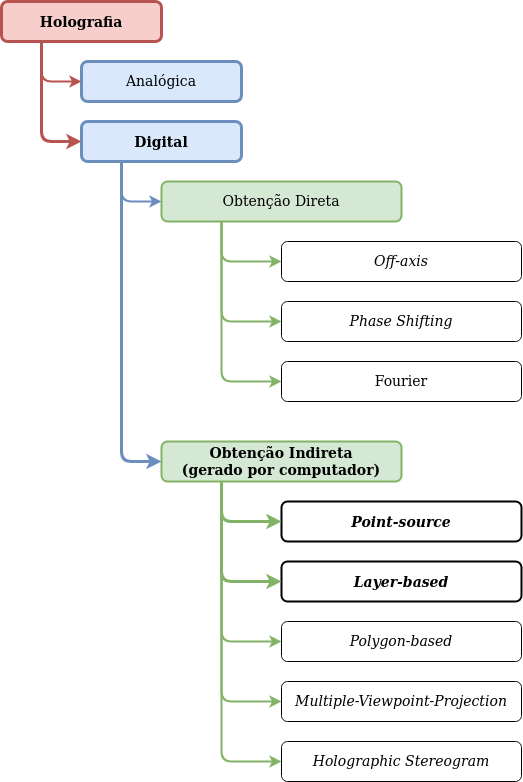
\includegraphics[width=.9\textwidth]{holografia}
  \caption[Métodos de obtenção de hologramas.]{Métodos de obtenção de hologramas\cite{Image2018}. A negrito estão destacados os métodos utilizados na obtenção dos hologramas testados no presente projeto.}
  \label{fig:holografia}
\end{figure}

\begin{figure}[!htbp]
  \centering
  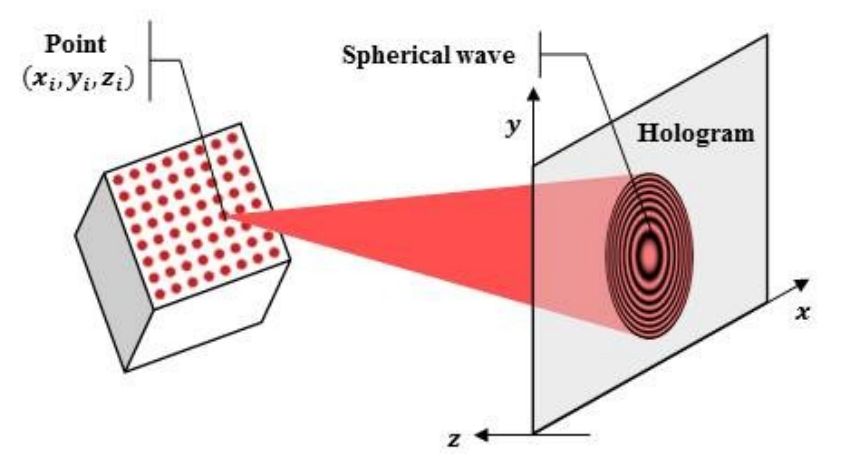
\includegraphics[width=.9\textwidth]{point-source}
  \caption[Obtenção de um \acs{HGC} pela técnica \textit{point-source}]{Obtenção de um \acs{HGC} pela técnica \textit{point-source}\cite{Image2018}.}
  \label{fig:point-source}
\end{figure}

\begin{figure}[!htbp]
  \centering
  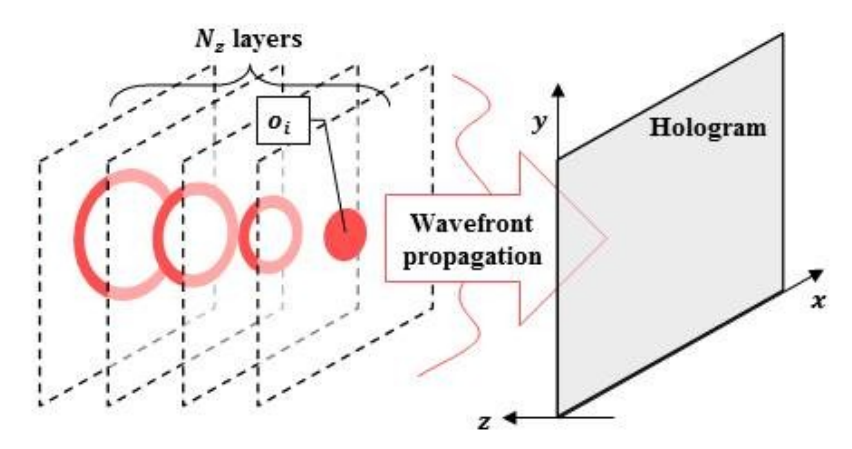
\includegraphics[width=.9\textwidth]{layer-based}
  \caption[Obtenção de um \acs{HGC} pela técnica \textit{layer-based}]{Obtenção de um \acs{HGC} pela técnica \textit{layer-based}\cite{Image2018}.}
  \label{fig:layer-based}
\end{figure}


\subsection{Reconstrução}
\label{ssec::estado-arte:holograma:reconst}

Esta fase do processo da holografia digital pode ser alcançada de duas formas\cite{Image2018}:
\begin{enumerate}
  \item \textbf{Reconstrução numérica}, onde é feita simulação da difração da luz por parte do holograma digitalmente obtido;
  \item \textbf{Reconstrução ótica}, com a propagação física de um feixe ótico com recurso a um \textit{laser} e a um \ac{SLM}.
\end{enumerate}

Apenas o primeiro tipo de reconstrução será abordado por ser o utilizado no projeto.

São então definidos três métodos de reconstrução numérica consoante a distância de reconstrução\cite{Image2018}:
\begin{enumerate}
  \item \ac{ASM} (curta distância);
  \item \ac{HCM} (média-longa distância);
  \item \ac{FTM} (longa distância).
\end{enumerate}

O que será utilizado no projeto é o método \textbf{\ac{ASM}}. Não sendo objetivo máximo deste Capítulo explanar em detalhe os conceitos teóricos inerentes a este método, segue-se um breve resumo para esclarecimento com as principais fórmulas que serão diretamente utilizadas no desenvolvimento de \textit{scripts} no âmbito da investigação.

% \subsubsection{\acf{ASM}}
% \label{sssec::estado-arte:holograma:reconst:asm}

A \textbf{reconstrução numérica} de um holograma consiste na propagação da amplitude complexa registada do objeto no plano da câmara digital relativa à sua posição original. Esta é feita com recurso à teoria de difração escalar (Figura \ref{fig:diffraction-theory})\cite{Image2018}, a qual estabelece que um campo difratado $\psi_p(x,y;z)$ pode ser obtido a partir do campo incidente $\psi_{p_0}(x,y)$ de acordo com a equação (\ref{eq:diffracted-field})\cite{Poon2014},

\begin{equation}
  \psi_p(x,y;z) = \mathcal{F}^{-1}\left\{\mathcal{F}\left\{\psi_{p_0}(x,y)\right\}\times\mathcal{H}(k_x,k_y;z)\right\}
  \label{eq:diffracted-field}
\end{equation}

onde $\mathcal{H}(k_x,k_y;z)$ é a \ac{SFTF} (equação (\ref{eq:stft})).

\begin{figure}[!bp]
  \centering
  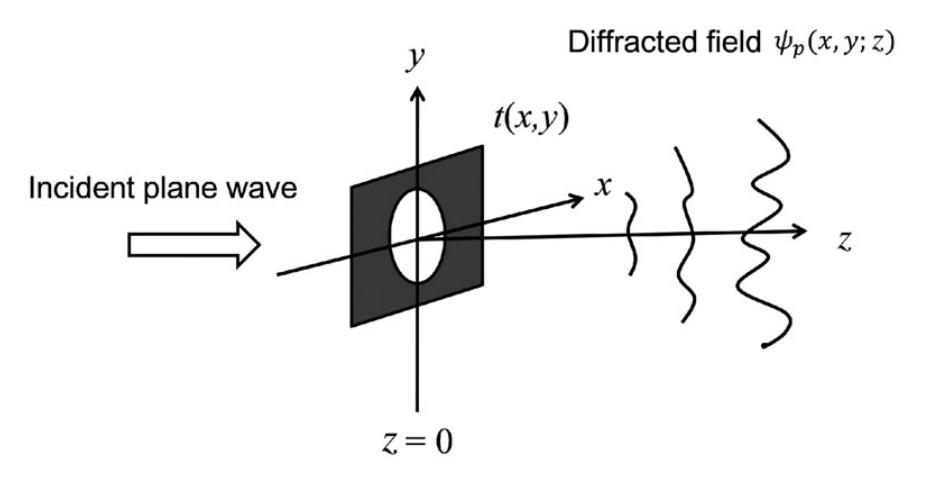
\includegraphics[width=.9\textwidth]{diffraction-theory}
  \caption[Geometria da difração.]{Geometria da difração, onde $t(x,y)$ é um ecrã de difração\cite{Poon2014}.}
  \label{fig:diffraction-theory}
\end{figure}

\begin{equation}
  \mathcal{H}(k_x,k_y;z) = \exp\left[2j\pi z\sqrt{\frac{1}{\lambda^2}-k_x^2-k_y^2}\right]
  \label{eq:stft}
\end{equation}

De notar que:
\begin{itemize}
  \item $\lambda$ é o comprimento de onda do feixe de luz;
  \item $\mathcal{F}$ é a Transformada de Fourier;
  \item $k_x$ e $k_y$ são as frequências espaciais radianas.
\end{itemize}

A equação (\ref{eq:diffracted-field}) é a fórmula de base do método \ac{ASM} (também conhecido por Método da Dupla Transformada de Fourier ou Método de Convolução)\cite{Poon2014}.


\subsection{Representação}
\label{ssec::estado-arte:holograma:rep}

Os dados holográficos podem ser representados de várias formas. Embora sejam todas equivalentes no sentido em que representam o mesmo objeto, algumas tornam a compressão mais eficiente. 

No âmbito deste projeto, apenas é relevante a representação no campo de onda complexo, o qual pode englobar\cite{Image2018}:

\begin{itemize}
    \item \textbf{Dados reais e imaginários}: utilizam um sistema de coordenadas cartesiano para representar amplitudes complexas;
    \item \textbf{Dados da amplitude e fase}: os valores complexos são expressos num sistema de coordenadas polares.
\end{itemize}

Os hologramas utilizados neste projeto são representados pelo formato de \textbf{amplitude-fase} (Figura \ref{fig:ampli-fase}).


\begin{figure}[!htbp]
  \centering
  \begin{tabular}{c c}
    \includegraphics[width=0.4\textwidth]{piano4k_ampli} &
    \includegraphics[width=0.4\textwidth]{piano4k_phase} \\
     Amplitude & Fase \\
  \end{tabular}
  \caption[Exemplo de um holograma no formato amplitude-fase]{Exemplo do holograma \texttt{piano4k} no formato amplitude-fase.}
  \label{fig:ampli-fase}
\end{figure}


\section{Compressão de um Holograma}
\label{sec::estado-arte:compress}


Dado que a dimensão dos ficheiros digitais pode ser avultada, tem sido do interesse da área da holografia estudar métodos eficientes de compressão que não comprometam a qualidade dos hologramas.

Neste sentido, o primeiro modelo de codificação e transmissão digital de hologramas foi proposto em 1991. Este envolvia a modulação dos dados num sinal de televisão com recurso a uma versão modificada do MPEG-2\cite{Sato1991}. 
Em 1993, o recurso aos formatos MPEG-1 e MPEG-2 foi novamente proposto para a compressão de segmentos do holograma correspondentes a diferentes perspetivas de reconstrução\cite{YOSHIKAWA1993,Yoshikawa1996}.

Contudo, apenas em 2002 foi concluído que os melhores rácios de compressão são esperados quando os hologramas digitais são representados pelas suas componentes real e imaginária de forma independente\cite{Naughton2002}.

Desde então vários estudos têm sido feitos no sentido de perceber os melhores métodos de compressão, incluindo estudos baseados na quantização escalar\cite{Arrifano}
e formatos com perda (\textit{e.g.} JPEG, JPEG2000, MPEG-4 AVC, Dirac e HEVC)\cite{Xing2014,Darakis2010,Peixeiro2016,Pinheiro2018}.

Sendo o formato JPEG2000 o investigado no presente projeto, este será seguidamente abordado.


\subsection{Uma Breve Introdução ao JPEG2000}
\label{ssec::estado-arte:compress:jpeg2000}

O formato JPEG2000 é uma norma internacional para a compressão de imagens. Esta foi elaborada com o objetivo de mitigar os problemas e as limitações enfrentadas com o formato \ac{JPEG} clássico de 1992. Uma das abordagens para alcançar este objetivo foi a substituição do uso de \ac{DCT} para um método baseado na transformada \textit{wavelet}\cite{Taubman2002}.

Conforme verificado pela Parte 1 da norma JPEG2000, algumas das vantagens a destacar são\cite{Pierre-AnthonyLemieux,Taubman2002}:
\begin{itemize}
  \item \textit{Eficiência de compressão}:\\ Em média \SI{20}{\percent} superior face ao \ac{JPEG} clássico.
  \item \textit{Escalabilidade da qualidade}:\\ Possibilidade de extrair praticamente qualquer qualidade reduzida.
  \item \textit{Escalabilidade da resolução}:\\ Possibilidade de extrair qualquer resolução que seja relacionada a uma potência de 2.
  \item \emph{Acessibilidade da \ac{ROI}}:\\ Habilidade de reconstruir uma região espacial arbitrária.
  \item \textit{Paralelismo}:\\ Capacidade de utilizar computação paralela com recurso a:
  \begin{itemize}
    \item Múltiplos \textit{cores} de uma \ac{CPU};
    \item Várias \textit{threads} numa \ac{GPU};
    \item \textit{Hardware} dedicado.
  \end{itemize}
  \item \textit{Controlo ótimo não-iterativo do rácio}:\\ Poder de alcançar um tamanho de compressão alvo sem recorrer a codificação iterativa.
\end{itemize}
% ISO/IEC JTC 1/SC 29/WG1 | Document N87018

Contudo, a norma JPEG2000 enfrenta como principal desvantagem o facto de ser computacionalmente bastante mais exigente, em especial com conteúdo de muito alta qualidade (\ac{UHD}).

A compressão nesta norma envolve várias fases, a saber\cite{Taubman2002a}:
\begin{enumerate}
  \item \textit{Transformada de cor}:\\ As imagens no formato \ac{RGB} são inicialmente transformadas num novo espaço de cor, havendo duas possibilidades para tal:
  \begin{enumerate}
    \item \acf{ICT}:\\ Transforma para o modelo YCbCr com recurso a números de vírgula flutuante ou de ponto fixo que geram erros de arredondamento (sendo assim chamado de ``irreversível'').
    \item \acf{RCT}:\\ Transforma para um modelo YUV modificado que não introduz erros de quantização (sendo, portanto, ``reversível''). As transformações são:\\
    \begin{tabular}{r @ {~=~} l @{~~;~~~~~} r @ {~=~}  l @{~;}}
      $Y$   & $\left\lfloor\frac{R+2G+B}{4}\right\rfloor$ & $G$ & $Y-\left\lfloor\frac{C_B+C_R}{4}\right\rfloor$ \\
      $C_B$ & $B-G$ & $R$ & $C_R+G$ \\
      $C_R$ & $R-G$ & $B$ & \multicolumn{1}{l @{~.}}{\hspace{-6pt}$C_B+G$} \\
    \end{tabular}
  \end{enumerate}
  
  \item Tiling:\\ A imagem é dividida em \textit{tiles}, \textit{i.e.} regiões retangulares que são codificadas separadamente. Cada \textit{tile} pode ter um tamanho qualquer, podendo a imagem completa ser, no limite, uma \textit{tile}. Todas as \textit{tiles} têm o mesmo tamanho. Esta fase pode introduzir o mesmo efeito de blocos encontrado na norma \ac{JPEG} clássica e pode ainda condicionar o valor de \ac{PSNR} da imagem comprimida.
  
  \item \textit{Transformada \emph{wavelet}}:\\ Cada \textit{tile} passa por uma transformada \textit{wavelet} de tamanho arbitrário (\textit{versus} o tamanho padrão de $8 \times 8$ do \ac{JPEG} clássico). Semelhante à transformada de cor, existem dois tipos de transformada \textit{wavelet}:
  \begin{enumerate}
    \item \textit{Irreversível}:\\ Introduz ruído de quantização.
    \item \textit{Reversível}:\\ Recorre exclusivamente a coeficientes inteiros, pelo que não é necessário arredondamento, prevenindo assim a inserção de ruído de quantização\cite{Bovik2009,LeGall,Unser2003}.
  \end{enumerate}
  
  \item \textit{Quantização}:\\ Os coeficientes passam por uma quantização escalar a fim de reduzir o número de \textit{bits} para os representar. O passo de quantização permite controlar a taxa de compressão: um maior passo de quantização aumenta a compressão, mas com a desvantagem natural de diminuir a qualidade final. Um passo de quantização unitário (\textit{i.e.} com valor $1$) leva a que este passo não seja sequer realizado.
  
  \item \textit{Codificação}:\\ Passo complexo que envolve um processo denominado \ac{EBCOT}. Os detalhes deste passo ultrapassam o âmbito do projeto.
\end{enumerate}

Os ficheiros resultantes têm tradicionalmente a extensão \verb|*.jp2|. Há ainda a referir o formato \verb|*.jpx| com o qual se podem incluir animações.

Por fim, os metadados de uma imagem codificada com a norma JPEG2000 são armazenados no formato \ac{XML}\cite{bib:jpeg2000}, contrastando com o formato tradicional \textit{Exif} utilizado pela norma \ac{JPEG} clássica e outras normas de compressão e armazenamento de multimédia.


\subsection{\acs{PSNR}: uma Métrica de Relação Qualidade-Débito}
\label{ssec::estado-arte:compress:psnr}

\textbf{\acf{PSNR}} é uma métrica utilizada na área da engenharia que calcula o rácio entre a potência máxima possível de um sinal e a potência de sinais de ruído que afetam a fiabilidade da sua representação. Esta é expressa em \acf{dB}. A fórmula do \ac{PSNR} é dada pela equação (\ref{eq:psnr})\cite{salomon2007data},

\begin{equation}
  \mathrm{PSNR} = 20\cdot\log\left(\mathrm{MAX}_I\right) - 10\cdot\log\left(\mathrm{MSE}\right)
  \label{eq:psnr}
\end{equation}

onde:
\begin{itemize}
  \item $\mathrm{MAX}_I$ é o valor máximo possível do píxel da imagem (para uma representação com $n$ \textit{bits}, o valor será dado por $2^n-1$);
  \item \ac{MSE} (\textit{i.e.} erro médio quadrado) é dado pela equação (\ref{eq:psnr-mse}):
    \begin{equation}
      \mathrm{MSE} = \frac{1}{mn}\sum_{i=0}^{m-1}\sum_{j=0}^{n-1}\left[I(i,j)-K(i,j)\right]^2
      \label{eq:psnr-mse}
    \end{equation}
\end{itemize}

Para multimédia codificada com 8 \textit{bits} de profundidade em formatos com perdas, o valor de \ac{PSNR} ronda tipicamente os \SI{30}{\decibel} a \SI{50}{\decibel}\cite{welstead1999fractal,barni2006document}.


\section{Conclusões}
\label{sec::estado-arte:conclusao}
Apesar da holografia ser uma área com décadas de história e pesquisa, esta ainda carece de normas bem estabelecidas a fim de tornar a sua manipulação, o seu estudo e o seu uso exequíveis de uma forma prática.

Assim, com base no conhecimento de interesse coletado acerca da holografia e da compressão de imagens, torna-se necessário definir quais os materiais, as ferramentas e as tecnologias necessárias para a concretização da investigação nesta área.
